\documentclass[
logosetup=topbar 
portrait,
%landscape,
a0paper%,
%draft
]
{baposter}
\usepackage{varwidth}
\usepackage{graphicx}
\usepackage{tikz,pgfplots}

\usepackage{relsize}
\usepackage[detect-weight]{siunitx}
 
\usepackage{booktabs}
\usepackage{amsmath}
\usepackage{float}
\usepackage{layouts}
\usepackage{multirow}
\usepackage{subfig}
\newcommand\e{\cdot 10^}
\setlength{\unitlength}{1.0cm}

\usepackage{xcolor,colortbl}

%\definecolor{hzbblue}{HTML}{0BA1E2}%{2E9EDC}%{1F95D6}
\definecolor{hzbblue}{RGB}{31,149,213}
\usepackage[scaled]{helvet}
\renewcommand*\familydefault{\sfdefault}
\usepackage[T1]{fontenc}

\renewcommand{\refname}{}

\usepackage{transparent}

\begin{document}
%
\begin{poster}{
grid=false,%true,
background=plain,
bgColorOne=white,
columns=3,
eyecatcher=true,
borderColor=hzbblue,
headerColorOne=white,
headershade=plain,
%headerColorTwo=hzbblue,
textborder=rounded,%none,%rectangle,
headerborder=open,
headershape=smallrounded,
headerfont=\bf\Large,
boxshade=none,
headerFontColor=hzbblue
}
{

\includegraphics[width=150pt]{berkeley/ucberkeleybluehex.pdf} 
}
{
\color{hzbblue}Streak camera System and Tune Resonance Tool
}
{
\color{hzbblue} L. Dovlatyan, M. Ries, P. Goslawski, and friends at HZB \\
\color{hzbblue} levondov@berkeley.edu
}
{

\includegraphics[width=100pt]{Pics/hzb_logo_clean.pdf} 
}
\headerbox{Introduction}{name=introbox,column=0,row=0,span=3}
{
\begin{tikzpicture}
\node at (1,5)[]{
\begin{varwidth}{13cm}
The \textbf{H}elmholtz-\textbf{Z}entrum \textbf{B}erlin is a facility that operates two synchrotron light sources: BESSY II and the MLS. One of the long term goals of this center is to continually make bunch lengths as short as possible in storage rings. A way to go about this is through lattice design by changing the momentum compaction factor. An important part of lattice design involves picking a good working point to avoid the tune resonances of the machine. A tune resonance program was therefore developed which can be used to view the current working point and resonance lines given only a few input parameters from the EPICS control systems.

\end{varwidth}};
\node at (0,1){
\begin{varwidth}{11cm}
In order to study shortest bunches, diagnostic tools are needed. A new streak camera was recently purchased for the MLS, and was setup at a beamline above the machine on the second floor. The setup proved to be quite a challenged because of the placement of the camera and beamline. An optical path that needed six degrees (x,x',y,y',z,z') of freedom was setup; this setup also provided the opportunity to operate the old streak camera along side the new camera simulatanously and compare measurements.
\end{varwidth}};

\node at (12.0,3) {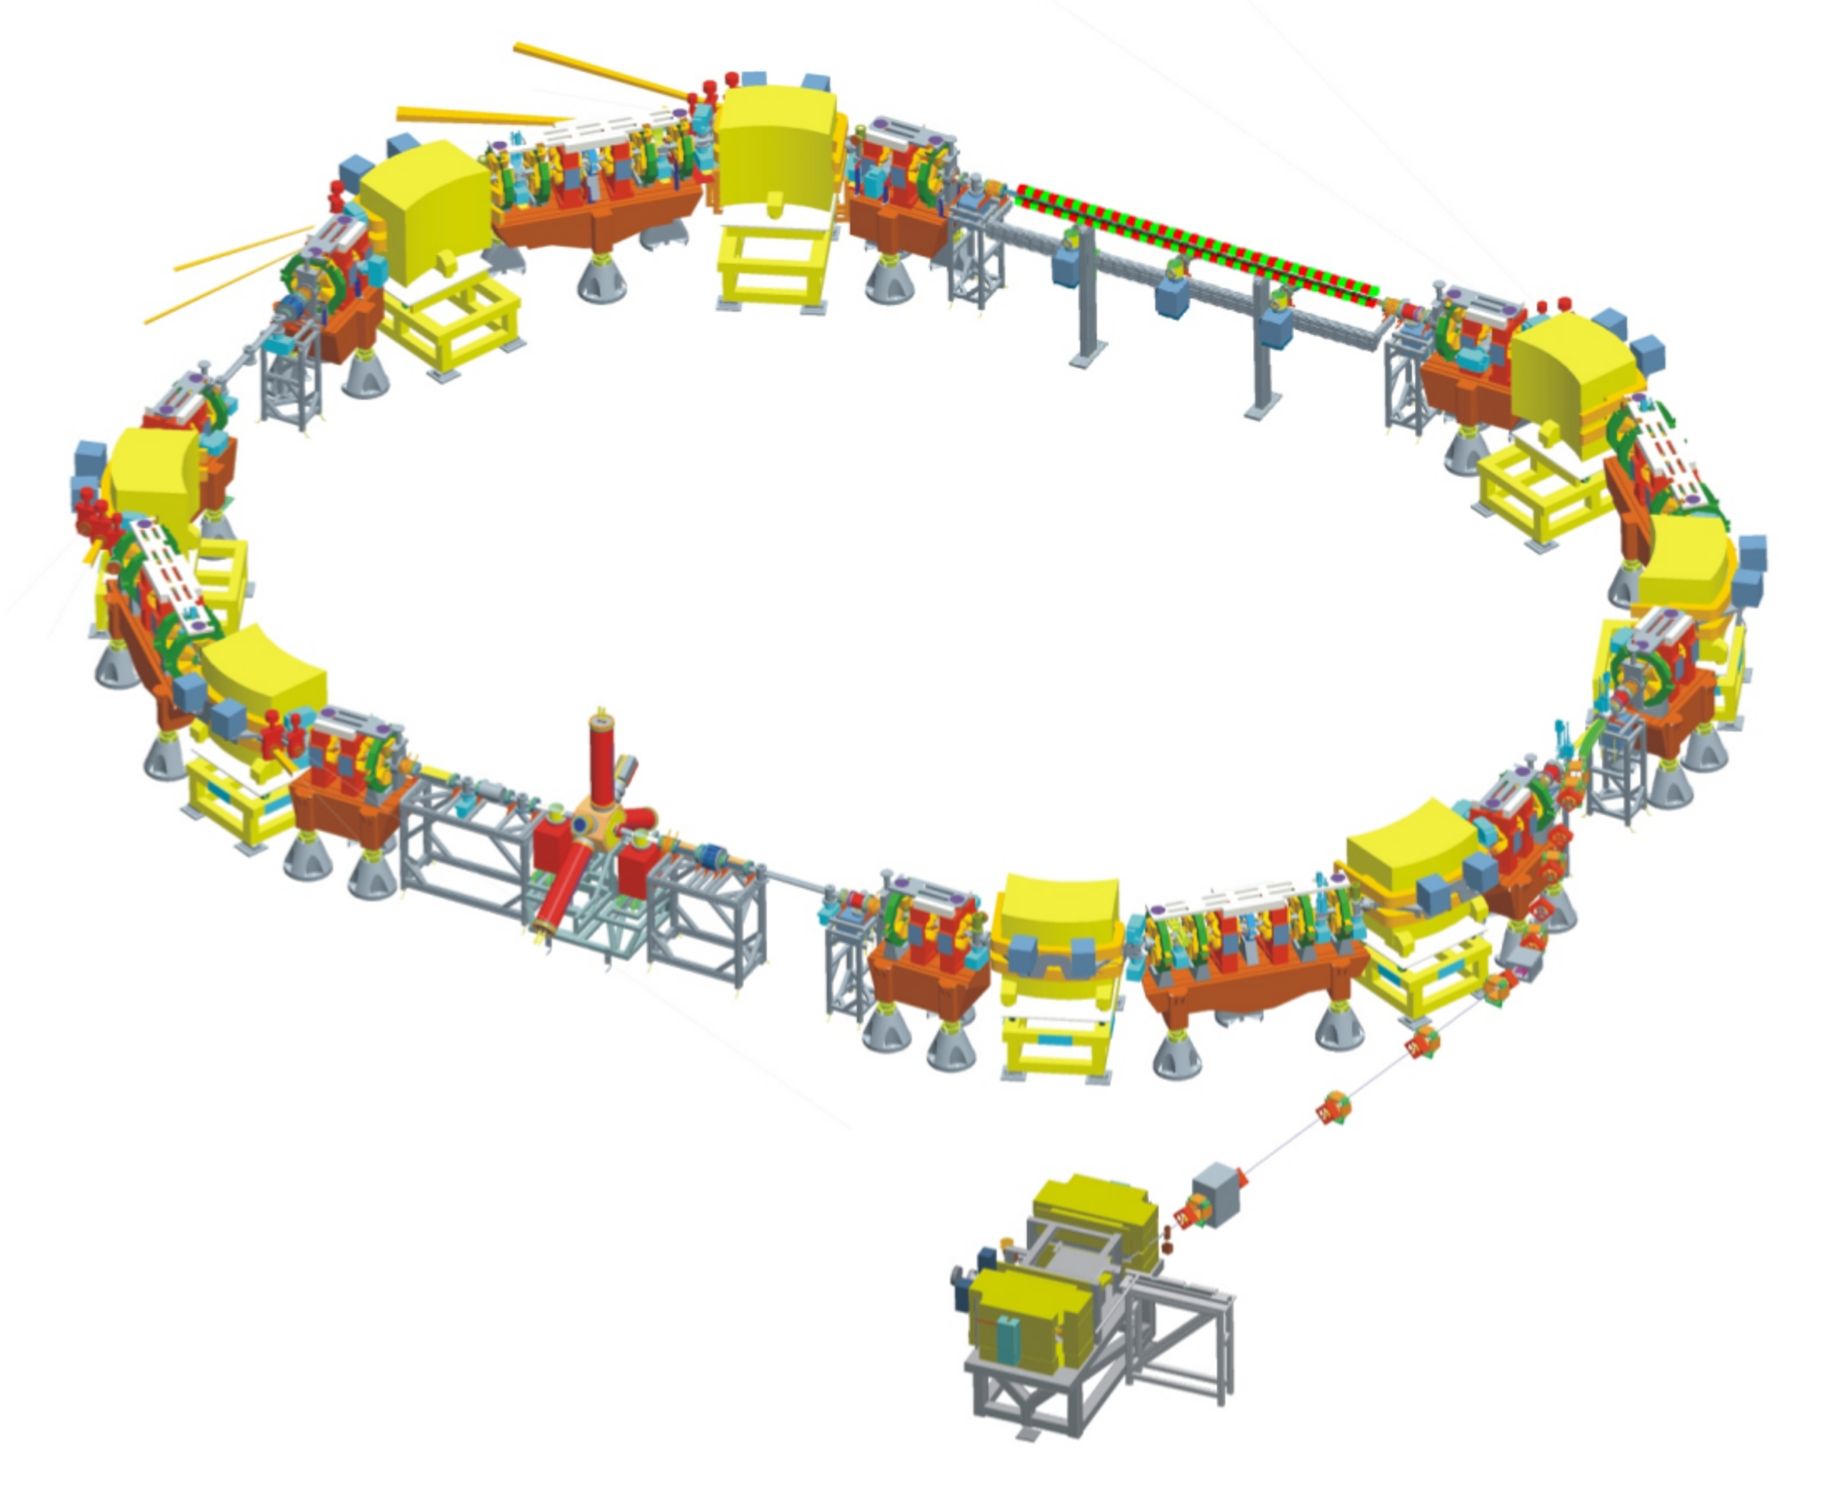
\includegraphics[width=250pt]{Pics/mls.pdf}};
\node at (9,0) {\footnotesize
\begin{tabular}{lc}%\hline
Lattice & {DBA}\\
Energy range / \si{\mega\electronvolt} &  105 to 630\\
Circumference / \si{\metre} &  48\\
Characteristic wavelength / \si{\nano\metre} &  3.4 to 735 \\
Tunes ver./hor. & {2.23 / 3.18}\\
Current$\times$Lifetime / \si{\ampere\hour}&  0.9  \\%\\\hline
electron beam current & 1 pA to 200 mA
\end{tabular}%
};
\node at (12,3.8){
\Huge\color{hzbblue} MLS
};
\draw [<-, rounded corners, thick, black] (10.8,6.5) -- (12.5,6.4);
\node at (14,6.4) {
beamline used
};
\node at (16, 0){
\includegraphics[width=75pt]{Pics/PTB-Logo.pdf}};
\end{tikzpicture}
}

\headerbox{Streak Camera Setup}{name=firstbox,below=introbox,column=0,row=1,span=2}
{
\begin{tikzpicture}

\node at (1,0.8) {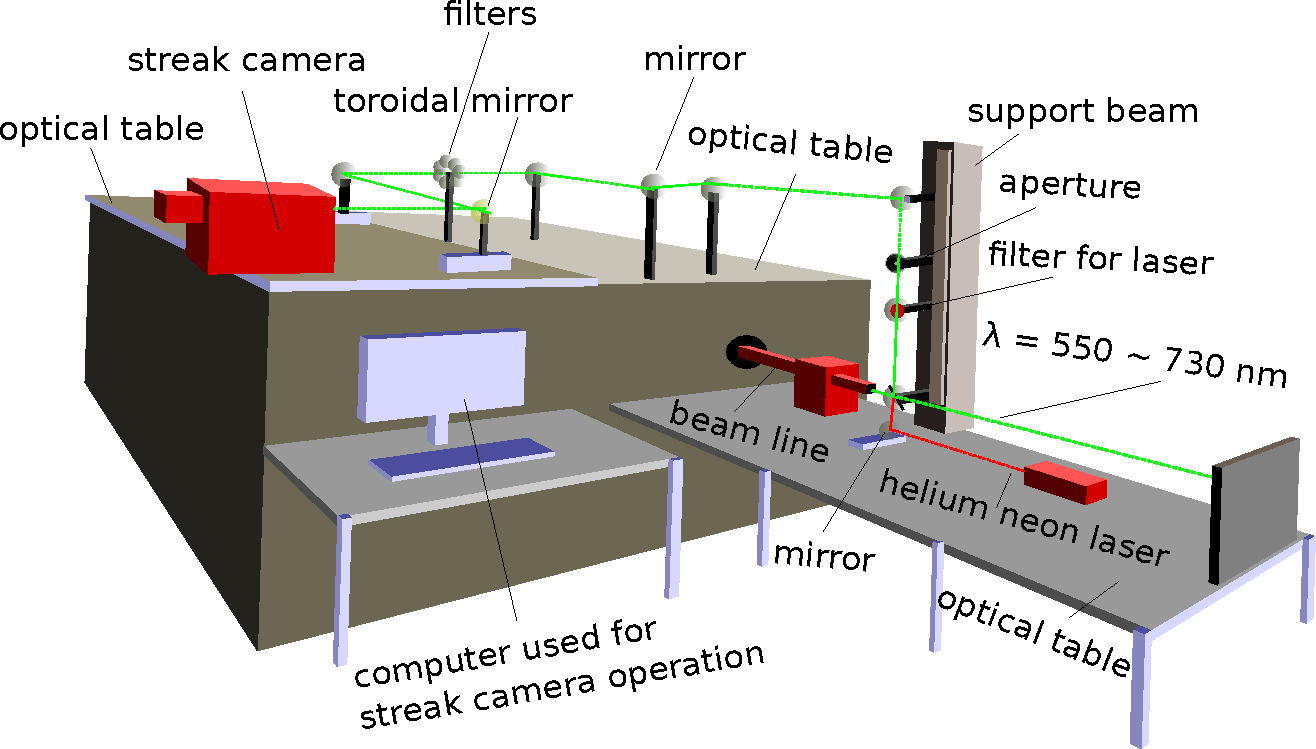
\includegraphics[width=300pt]{Pics/diagramtext.pdf}
};
\node at (8.7,1) {\fbox{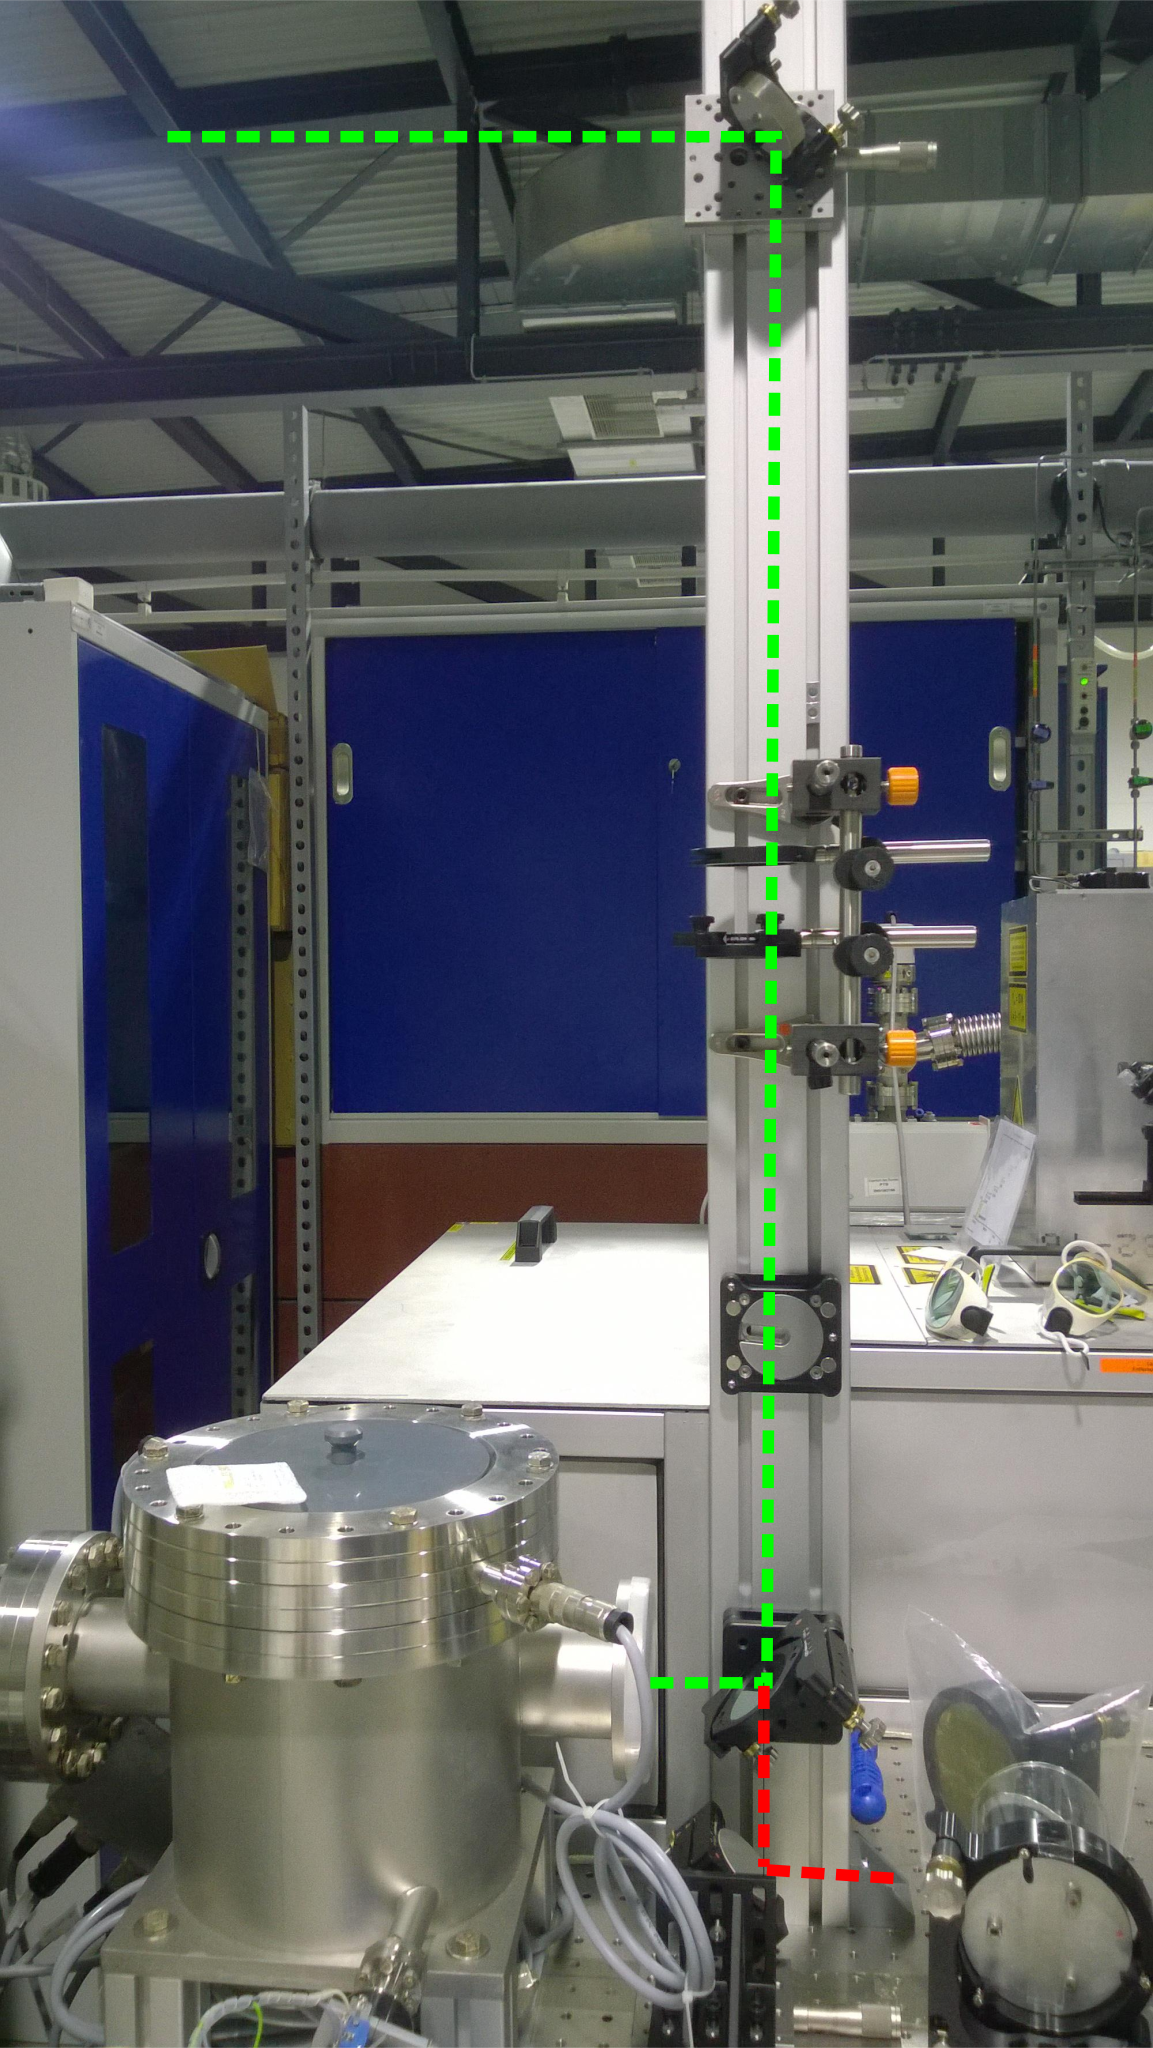
\includegraphics[width=90pt]{Pics/verticalbeam.pdf}}
};
\node at (6,-4.8) {\fbox{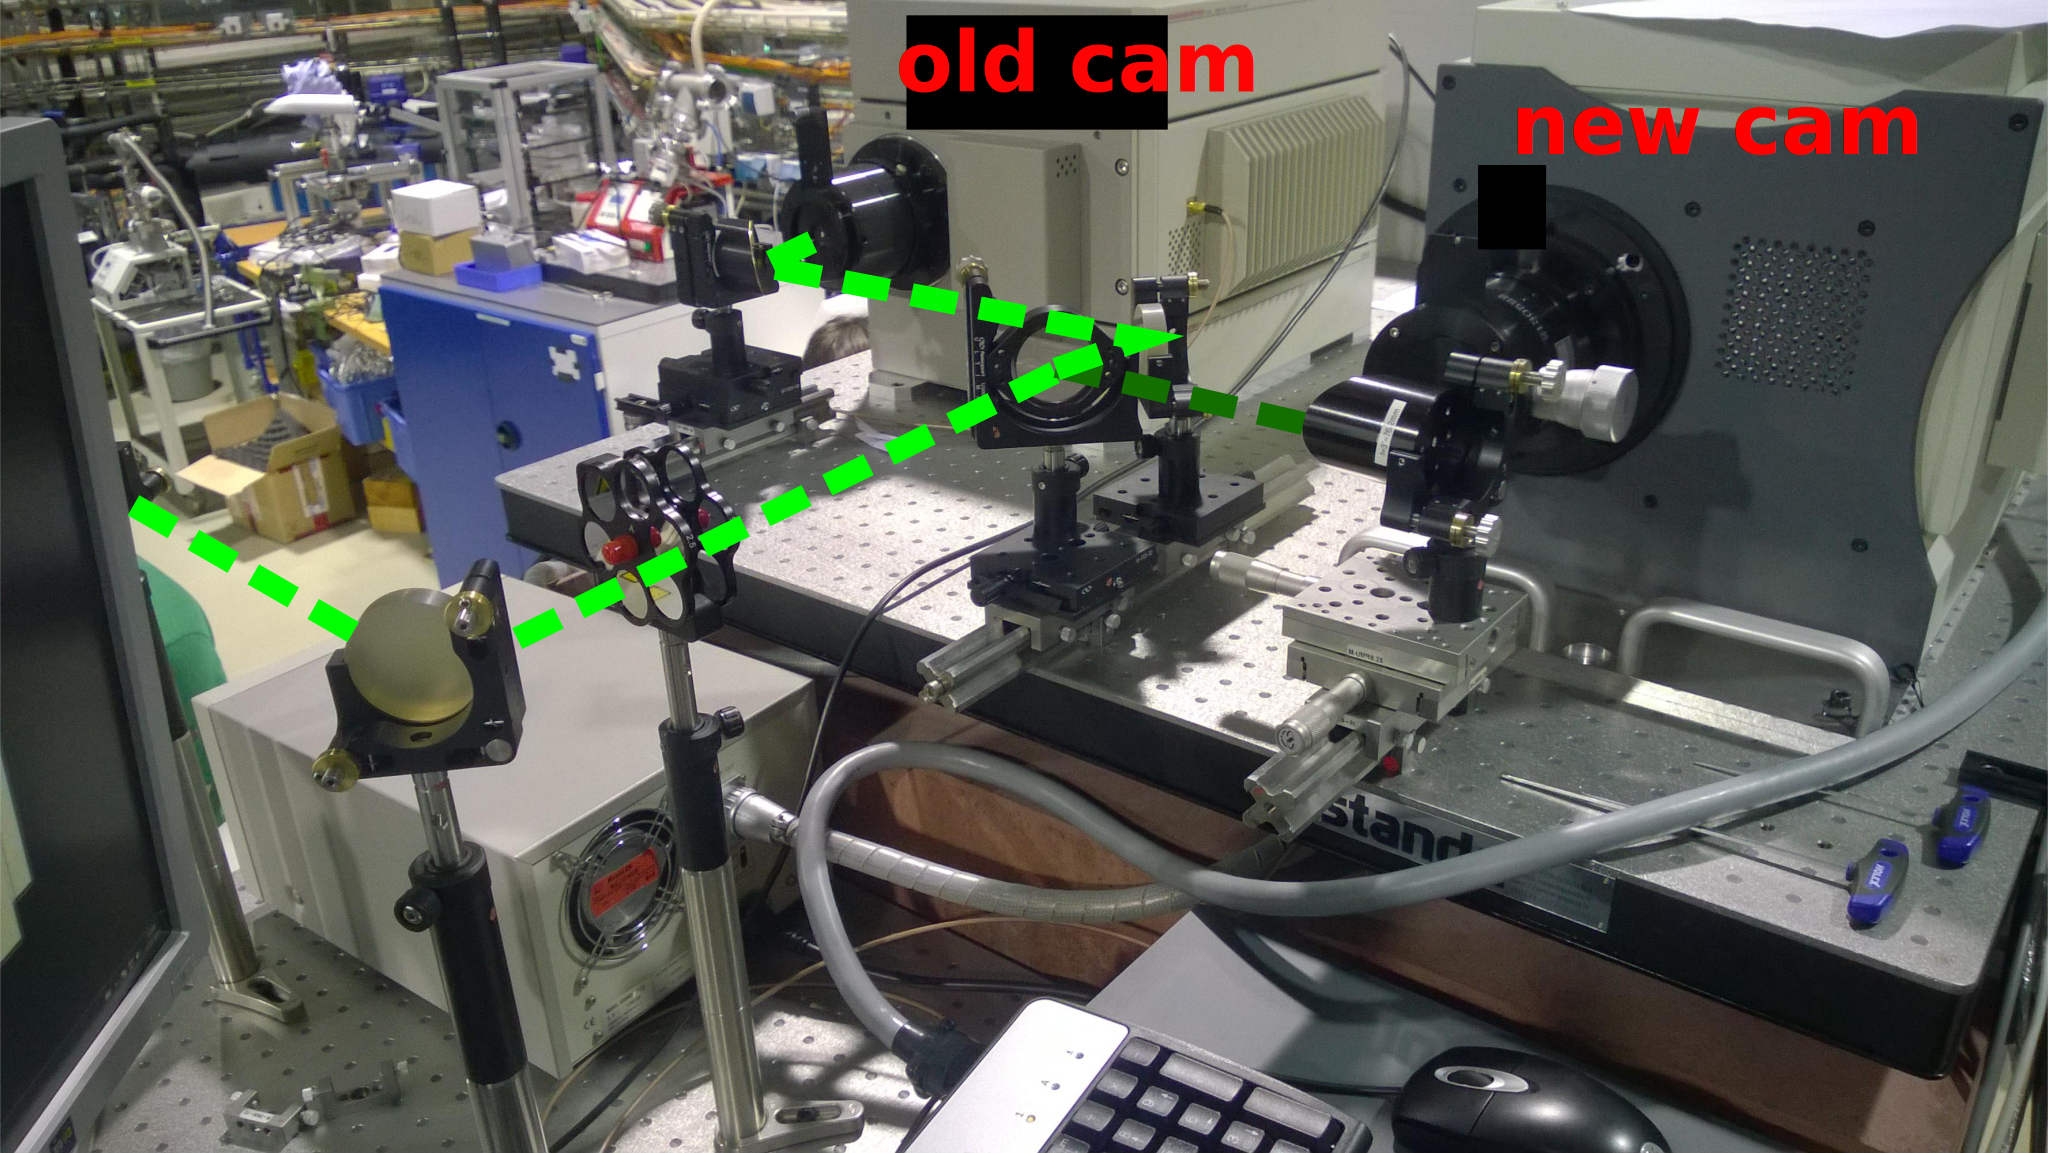
\includegraphics[width=175pt]{Pics/horizontaltable.pdf}}
};
\node at (6,-2.7) {
dual streak camera operation
};
\node at (8.7,-2.15) {
support beam
};
\node at (-1,-4.2) {
\begin{varwidth}{7cm}
The toroidal mirrors, along with a splitter and a plane mirror, on the optical table are placed on rail systems in order to provide multiple degrees of freedom to adjust for the horizontal and vertical focuses of the beam
\end{varwidth}
};
\end{tikzpicture}
}

\headerbox{Streak Camera Measurements}{name=secondbox,below=firstbox,column=0,row=2,span=2,above=bottom}
{
\begin{tikzpicture}[]


\node at (0,4.3) {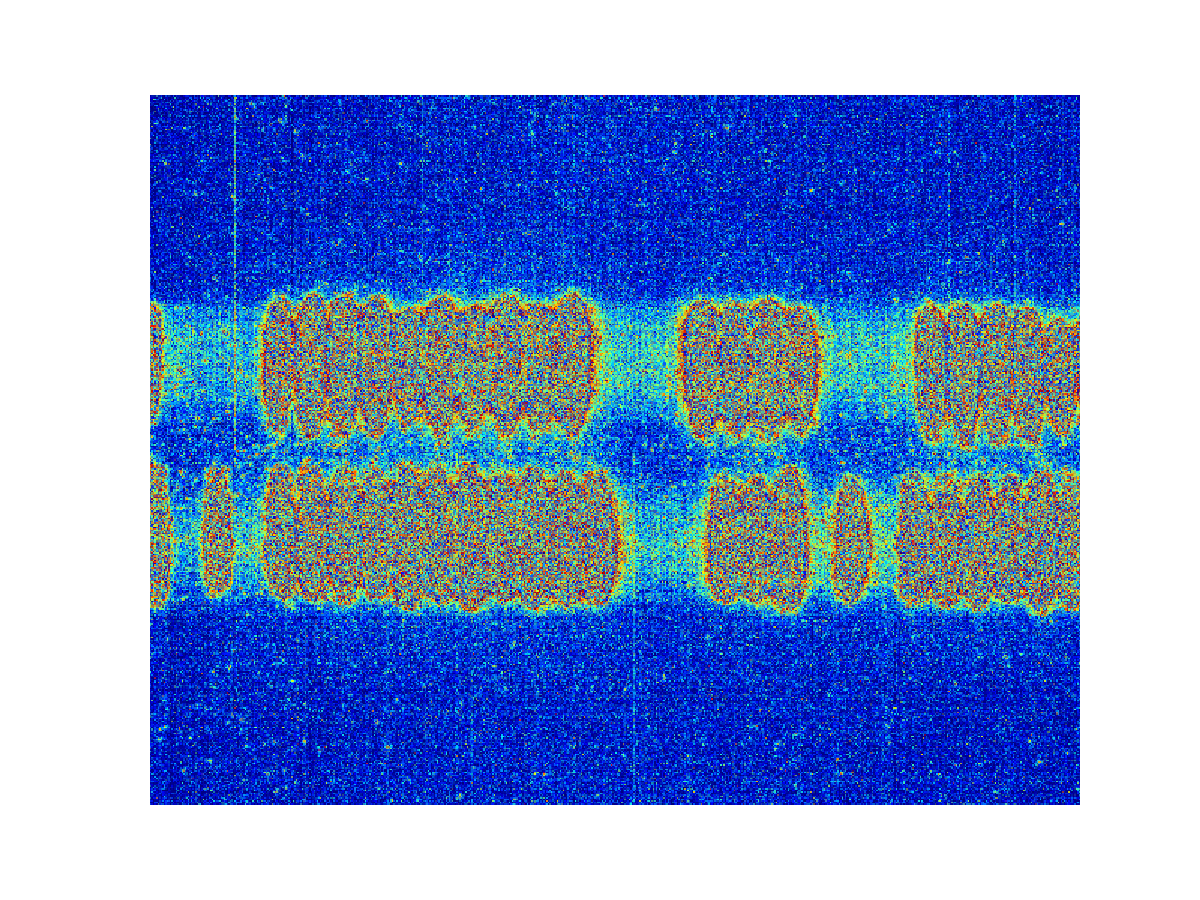
\includegraphics[height=175pt]{IP/levon/lowalpha_100mA_zerisseneFuellungmitLuecke.pdf}
};
\node at (0,4.3) {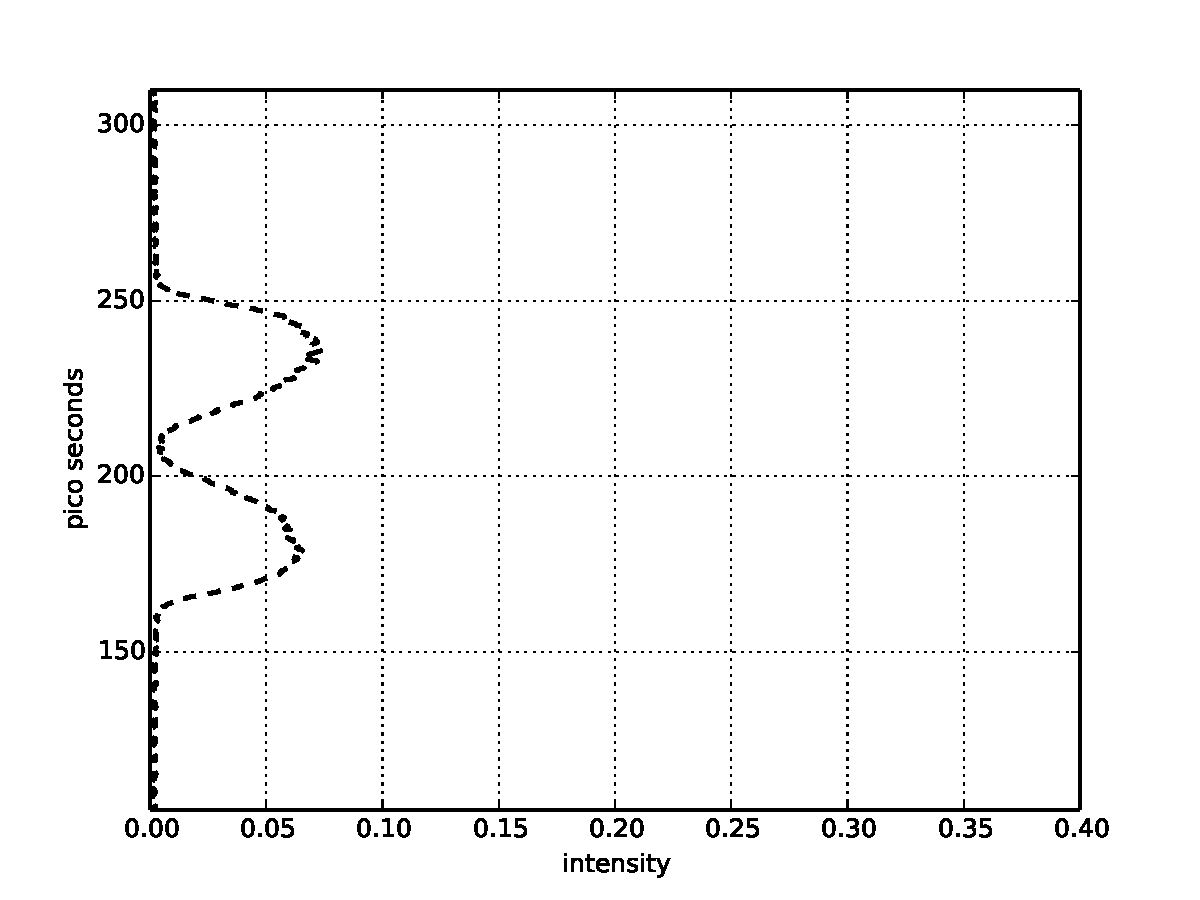
\includegraphics[height=175pt]{IP/levon/lowalpha_100mA_zerisseneFuellungmitLueckegraph.pdf}
};
\node at (7,4.3) {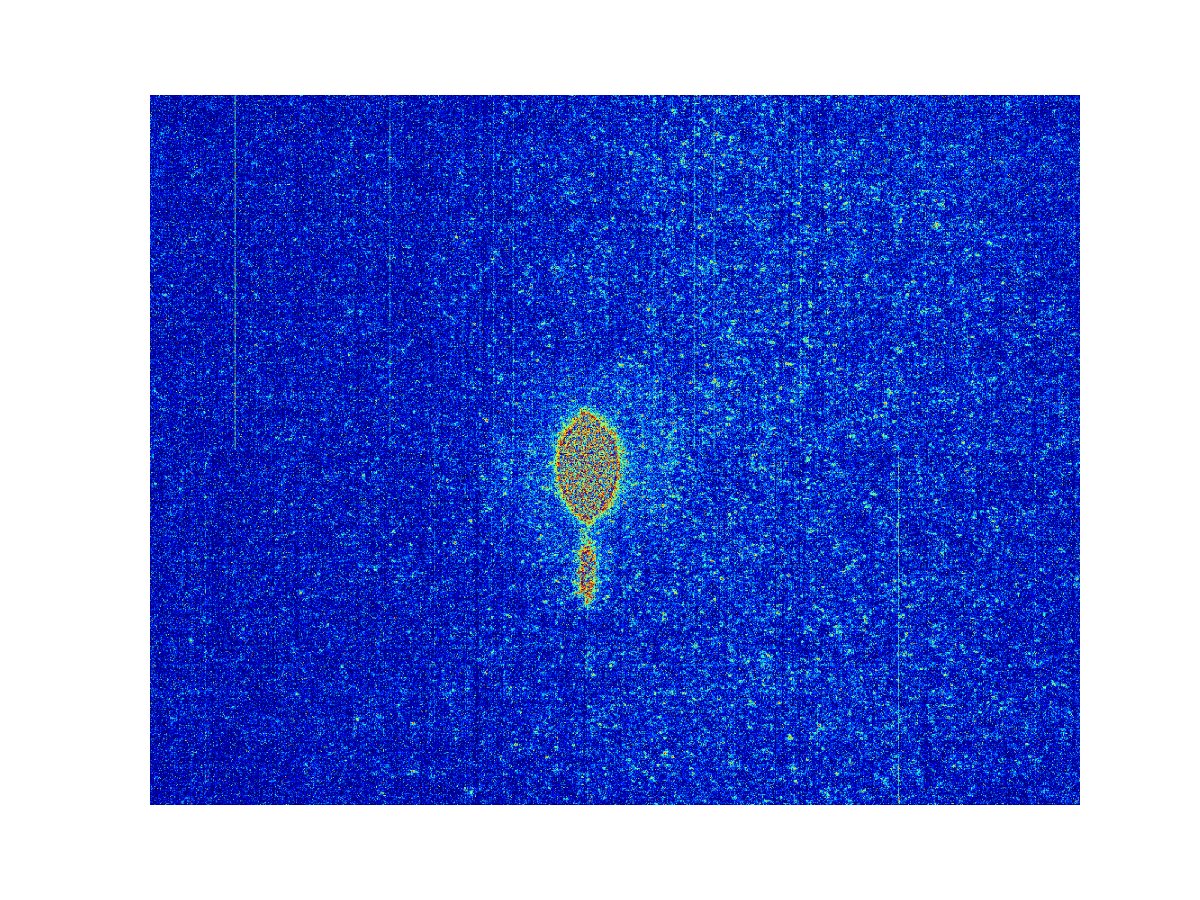
\includegraphics[height=175pt]{IP/levon/lowalpha_1uA.pdf}
};
\node at (7,4.3) {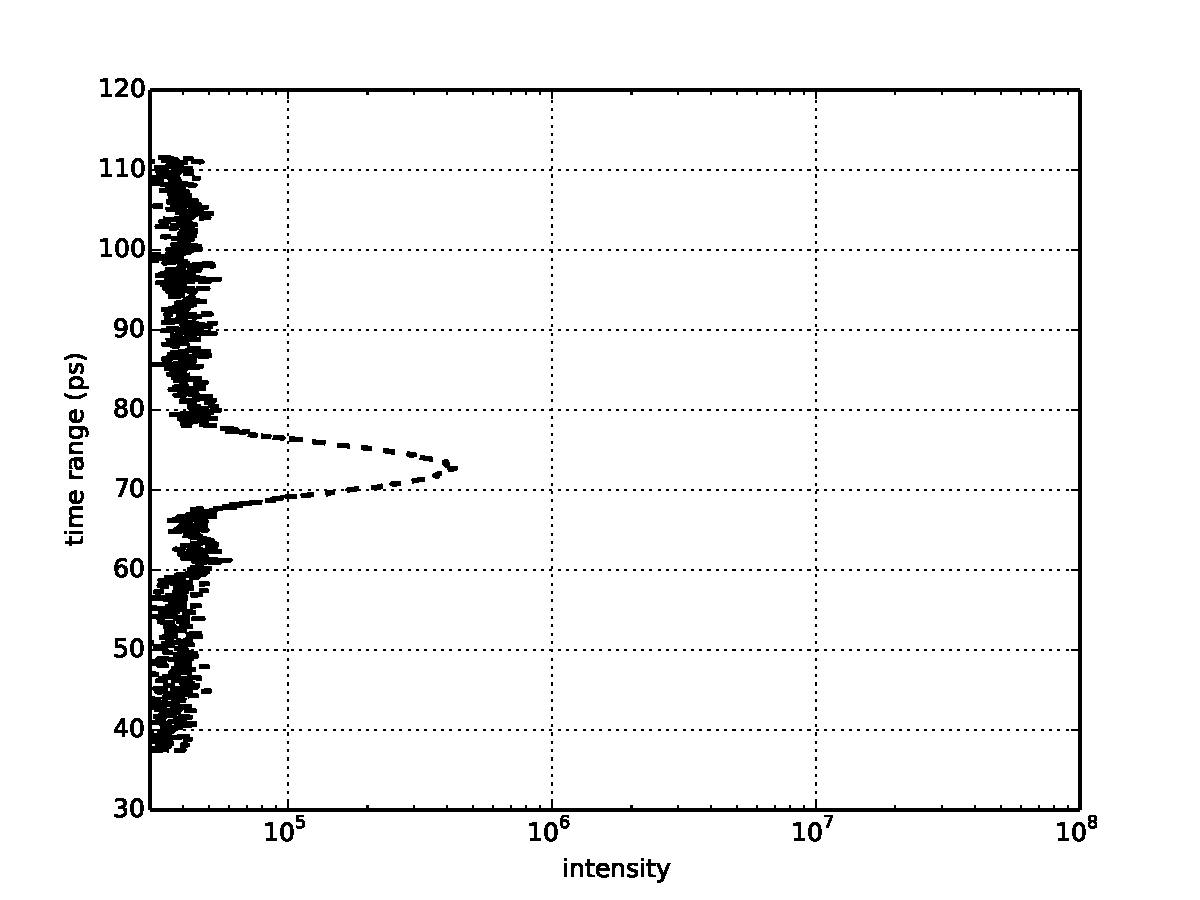
\includegraphics[height=175pt]{IP/levon/lowalpha_1uAgraph.pdf}
};
\node at (0,1) {
\large horizontal bunch length
};
\node at (7,1) {
\large single bunch measurement
};
\draw[<-,thick] (-2.95,5) to [out=90,in=180] (-2.5,7);
\draw[<-,thick] (1.55,5) to [out=90,in=0] (0.4,7);
\node at (-1,7) { \large one revolution
};
\draw [->, rounded corners, thick, black] (10,7) -- (7,3.5);
\node at (9.5,7.9) {
\begin{varwidth}{3.5cm}
possibly a reflection from inside the camera back onto the fluorescent screen
\end{varwidth}
};
\node at (3,8) {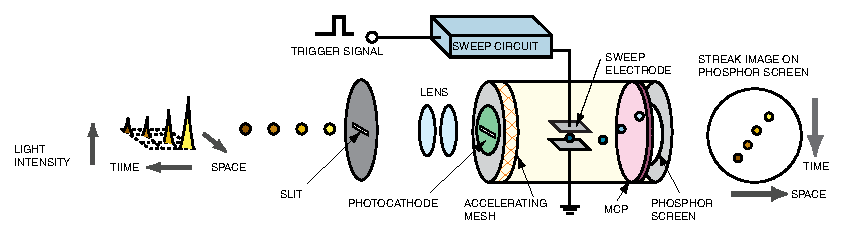
\includegraphics[width=250pt]{Pics/streakdiagram.pdf}};
\end{tikzpicture}
\node at (1,8) {\fbox{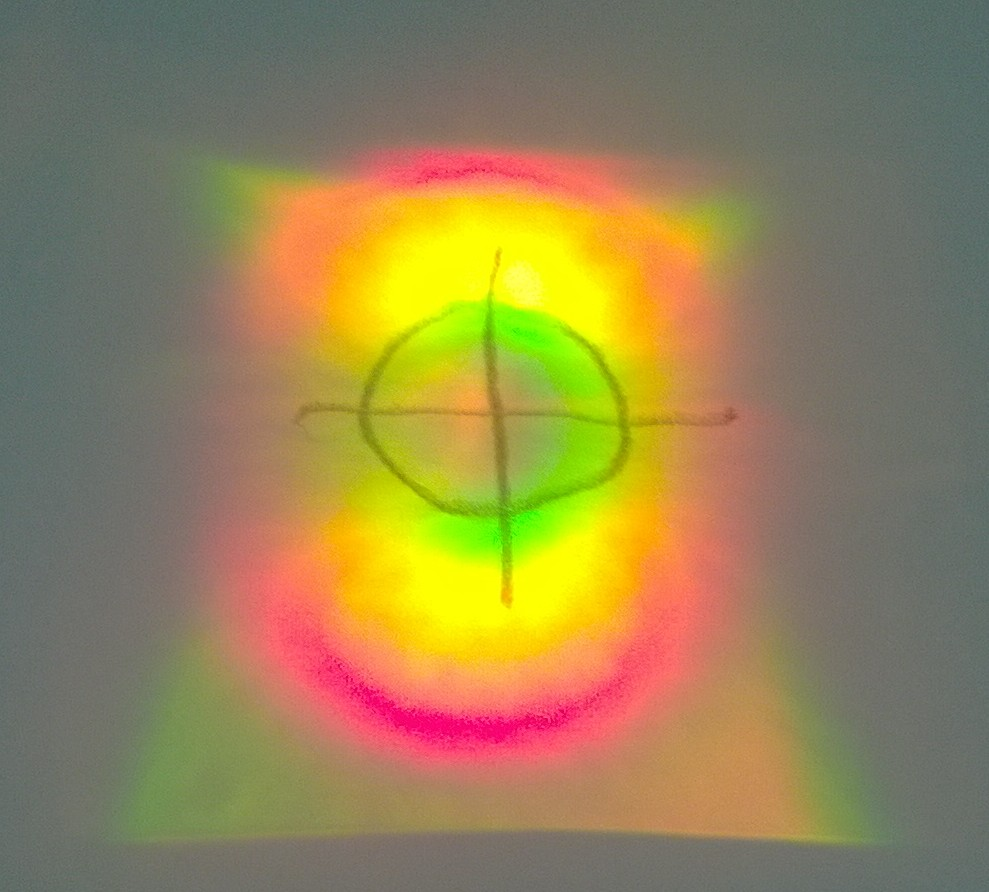
\includegraphics[width=50pt]{Pics/beam.jpg}}};
\draw [<-, rounded corners, thick, black] (2.2,8) -- (3.3,8.3);
\node at (3,8.5) {
image of beam
};
}

\headerbox{Tune Resonance Program}{name=tunediag,below=introbox,column=2,row=1,span=1,above=bottom}
{
{\color{hzbblue}\bf\large Details \& Features}
\begin{center}
\large Third order structural and phase advance resonance lines for the MLS
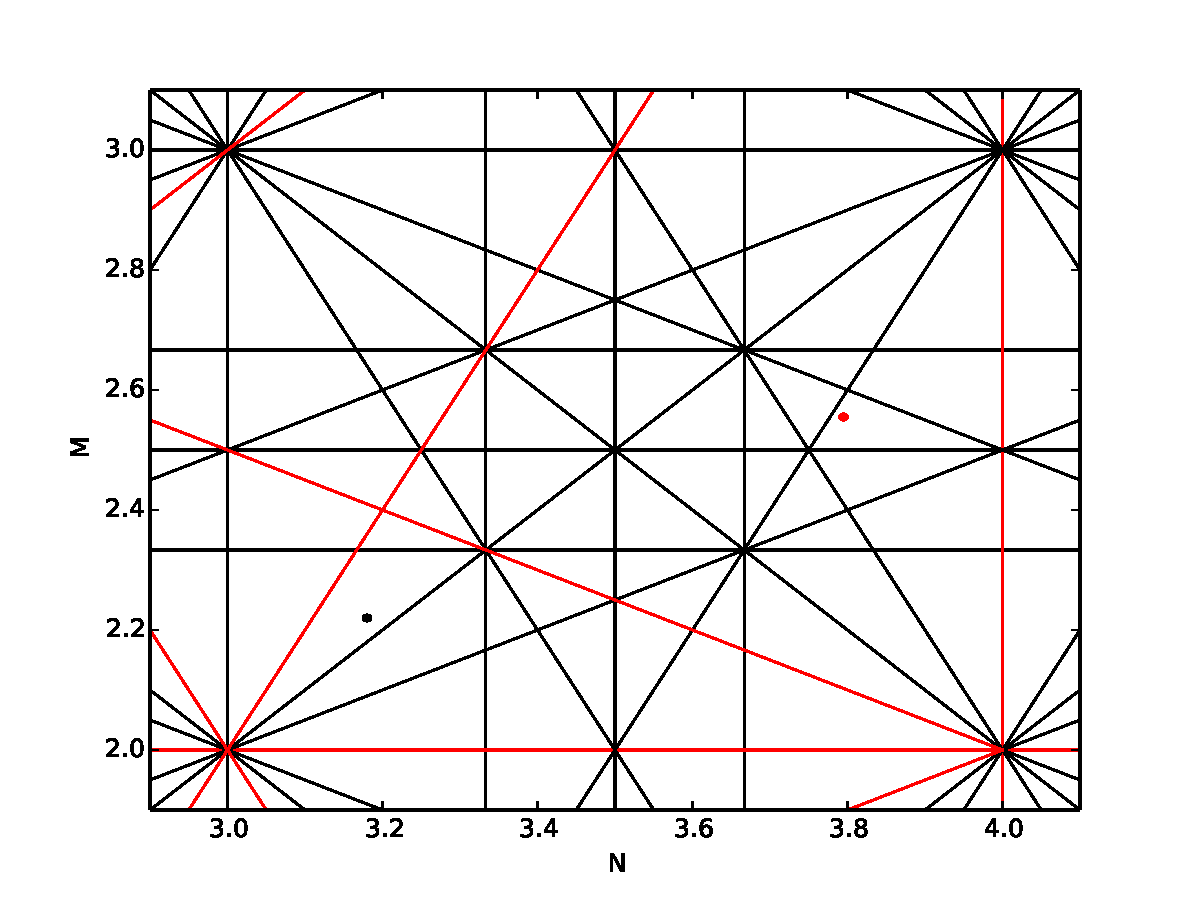
\includegraphics[width=200pt]{Pics/image.pdf}
\large Fifth order difference resonance lines ordered by color
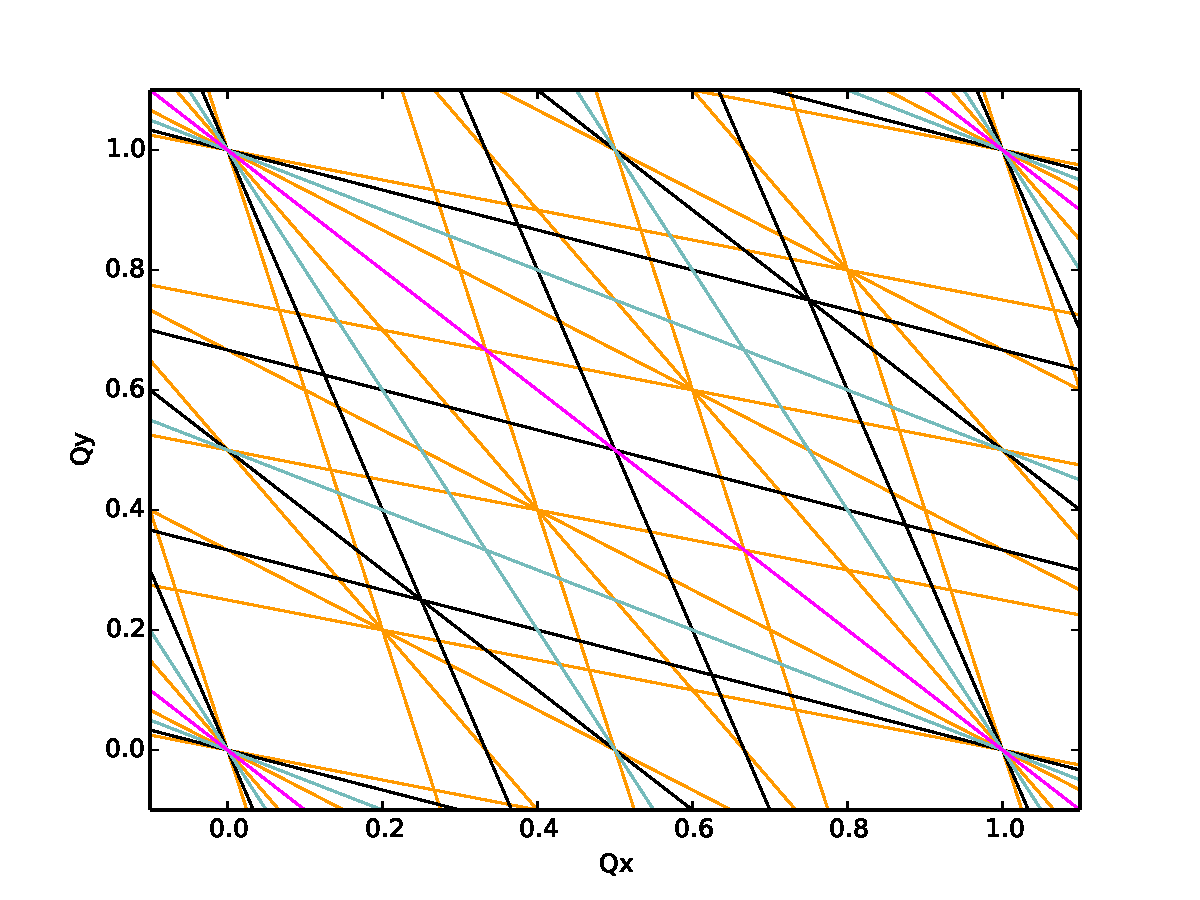
\includegraphics[width=200pt]{Pics/image2.pdf}
\end{center}

{\color{hzbblue}\bf\large Pictures \& Examples}
\begin{itemize}

\item[\color{hzbblue}\textbullet] developed in python
\item[\color{hzbblue}\textbullet] contains GUI built with wxpython
\item[\color{hzbblue}\textbullet] integrated with EPICS through the use of pyepics
\item[\color{hzbblue}\textbullet] live mode that displays current non-integer working point
\item[\color{hzbblue}\textbullet] given integer part, can display phase advance resonance lines and unit working point
\item[\color{hzbblue}\textbullet] various customizability options available

\end{itemize}
}
\end{poster}
\end{document}
